\documentclass[UTF8,a4paper,12pt]{ctexbook} 

 \usepackage{graphicx}%学习插入图
 \usepackage{verbatim}%学习注释多行
 \usepackage{booktabs}%表格
 \usepackage{geometry}%图片
 \usepackage{amsmath} 
 \usepackage{amssymb}
 \usepackage{listings}%代码
 \usepackage{xcolor}  %颜色
 \usepackage{enumitem}%列表格式
 \CTEXsetup[format+={\flushleft}]{section}


\geometry{left=1.6cm,right=1.8cm,top=2cm,bottom=1.7cm} %设置文章宽度

\pagestyle{plain} 		  %设置页面布局
\author{\kaishu 郑华}
\title{\heiti ACE 网络库学习笔记}
 %代码效果定义
 \definecolor{mygreen}{rgb}{0,0.6,0}
 \definecolor{mygray}{rgb}{0.5,0.5,0.5}
 \definecolor{mymauve}{rgb}{0.58,0,0.82}
 \lstset{ %
 	backgroundcolor=\color{white},   % choose the background color
 	basicstyle=\footnotesize\ttfamily,        % size of fonts used for the code
 	%stringstyle=\color{codepurple},
 	%basicstyle=\footnotesize,
 	%breakatwhitespace=false,         
 	%breaklines=true,                 
 	%captionpos=b,                    
 	%keepspaces=true,                 
 	%numbers=left,                    
 	%numbersep=5pt,                  
 	%showspaces=false,                
 	%showstringspaces=false,
 	%showtabs=false,        
 	columns=fullflexible,
 	breaklines=true,                 % automatic line breaking only at whitespace
 	captionpos=b,                    % sets the caption-position to bottom
 	tabsize=4,
 	commentstyle=\color{mygreen},    % comment style
 	escapeinside={\%*}{*)},          % if you want to add LaTeX within your code
 	keywordstyle=\color{blue},       % keyword style
 	stringstyle=\color{mymauve}\ttfamily,     % string literal style
 	frame=single,
 	rulesepcolor=\color{red!20!green!20!blue!20},
 	% identifierstyle=\color{red},
 	language=c++,
 }

\begin{document}          %正文排版开始
 	\maketitle
	\tableofcontents
\chapter{ACE概述}
	\section{OS适配层}
		OS适配层是位于本地OS API和ACE之间的“瘦”代码层,它使ACE的较高层与平台依赖性屏蔽开来,从而使得通过ACE编写的代码保持了相对的平台无关性。只需要极少的努力,开发者就可以将ACE应用移植到任何平台上。
		
	\section{C++包装层}
		C++包装层包括一些C++包装类,它们可用于构建高度可移植的和类型安全的C++应用。这是ACE工具包最大的一部分,大约包含了总源码的50\%。C++包装类可用于:
		
		\begin{enumerate}
			\item \textbf{并发和同步}:ACE提供若干并发和同步包装类,对本地OS多线程和多进程API进行了抽象.这些包装类封装用于线程和进程的原语,比如信号量、锁、栅栏(Barrier)和条件变量。另外还有更高级的原语可用,比如守卫(Guard)。所有这些原语共享类似的接口,因而很容易使用和相互替换。
			
			\item \textbf{IPC}:ACE提供若干C++包装类,封装不同OS中\textbf{不同的进程间通信}(IPC)接口。例如,ACE的包装类封装了以下IPC机制:BSD socket、TLI、UNIX FIFO、流管道、Win32命名管道,等等。ACE还为消息队列提供包装类,包括特定的实时OS的消息队列
			
			\item \textbf{内存管理组件}:ACE包含的一些类可用于内存动态分配和释放;其中包括允许预分配所有动态内存的类。这些预分配的内存随即通过ACE提供的管理类的帮助进行本地管理。在大多数实时和嵌入式系统中,这样的细粒度管理极为必要。另外还有一些类用于灵活地管理进程间共享内存。
			
			\item \textbf{定时器类}:有多种不同的类可用于处理定时器的调度和取消。ACE中不同种类的定时器使用不同的底层机制(堆、定时器轮(timer wheel)或简单列表)来提供不同的性能特性
			
			\item \textbf{容器类}:ACE还拥有若干可移植的STL风格的容器类,比如Map、Hash\_Map、Set、List,等等
			
			\item \textbf{信号处理}:ACE提供对特定OS的信号处理接口进行封装的包装类。这些类使得开发者能够很容易地安装和移除信号处理器,并且可以为一个信号安装若干处理器。另外还有信号守卫类,可用于在看守的作用域之内禁止所有信号
			
			\item \textbf{文件系统组件}:ACE含有包装文件系统API的类。这些类包括文件I/O、异步文件I/O、文件加锁、文件流、文件连接包装,等等
			
			\item \textbf{线程管理}:ACE提供包装类来创建和管理线程。这些包装还封装了针对特定OS的线程API,可被用于提供像线程专有存储这样的功能
		\end{enumerate}
	\section{框架模式层}
		ACE框架组件是ACE中最高级的“积木”,它们的基础是若干针对特定通信软件领域的设计模式。设计者可以使用这些框架组件来帮助自己在高得多的层面上思考和构建系统。这些组件实际上为将要构建的系统提供了“袖珍体系结构”,因此这些组件不仅在开发的实现阶段、同时在设计阶段都是有用的。ACE的这一层含有以下一些大型组件:
		
			\begin{enumerate}
				\item \textbf{事件处理}:大多数通信软件都\textbf{含有大量处理各种类型事件}(比如,基于I/O、基于定时器、基于信号和基于同步的事件)\textbf{的代码}。软件必须高效地多路分离、分派和处理这些事件。\textit{遗憾的是,大多数时间开发者们都在反复地编写这些代码,“重新发明轮子”}。这是因为,事件多路分离、分派和处理代码全都紧密地耦合在一起,无法彼此独立地使用。\textbf{ACE提供了被称为Reactor(反应器)的框架组件来解决这一问题}。\underline{反应器}\textit{提供用于高效地进行事件多路分离和分派的代码},并\textbf{极大地降低了它们与处理代码之间的耦合},从而改善了可复用性和灵活性。
				
				\item \textbf{连接或服务初始化组件}:ACE提供Connector(连接器)和Acceptor(接受器)组件,\textit{用于降低连接初始化与连接建立后应用执行的实际服务之间的耦合}。在接受大量连接请求的应用服务器中,该组件十分有用。\textbf{连接首先以应用特有的方式初始化,然后每一连接被相应的处理例程分别处理}。这样的去耦合使得开发者能够分别去考虑连接的处理和初始化。因此,\textbf{如果在随后的阶段开发者发现连接请求数多于或是少于估算,它可以选择使用不同的初始化策略集(ACE提供了若干可供开发者挑选和选择的策略),以获得所要求的性能水平}。
				
				\item \textbf{流组件}:ACE Stream组件用于简化那些本质上是分层的(layered)或层次的(hierarchic)软件的开发。用户级协议栈的开发是一个好例子;这样的栈由若干互连的层次组成。\textbf{这些层次或多或少可以相互独立地进行开发}。\textit{当“数据”通过时},每一层都处理并改变它,并将它传递给下一层,以作进一步的处理。\textbf{因为各层是相互独立的,它们很容易被复用或替换}。
				
				\item \textbf{服务配置组件}:通信软件开发者面临的另一个问题是,很多时候,软件服务必须在安装时配置,或必须在运行时重配置。应用中特定服务的实现可能需要进行改动,因而应用可能必须用新改动的服务重新配置。ACE Service Configurator(服务配置器)为应用的服务提供动态的启动、挂起和配置。
				
				\item \textbf{Task 组件}:Task框架,主要用于多线程的并发编程
			\end{enumerate}
	


\chapter{网络连接框架} 
	\section{类图概要} 
		根据底层使用的不同IPC接口,IPC\_SAP类被划分为四种主要的类属,图\ref{fig:IPC_SAP}描述了这一划分。ACE\_IPC\_SAP类提供的一些函数是所有IPC接口公有的。有四个不同的类由此类派生而出,每个类各自代表ACE包含的一种IPC\_SAP包装类属。这些类封装适用于特定IPC接口的功能。例如,ACE\_SOCK类包含的功能适用于BSD socket编程接口,而ACE\_TLI包装TLI编程接口。 
		
		\begin{figure}[h]
			\centering
			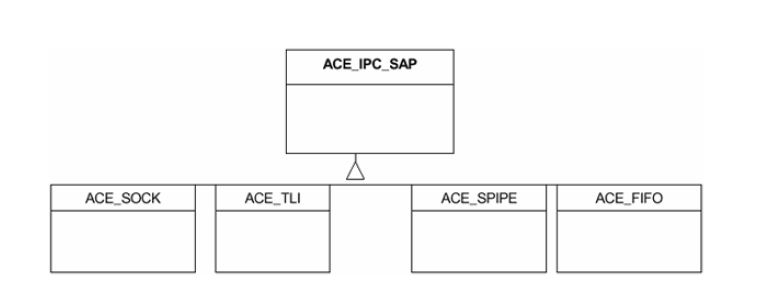
\includegraphics[width = 12cm]{IPC_SAP.png}
			\label{fig:IPC_SAP}
			\caption{IPC SAP 类属}
		\end{figure}  
		
	\section{socket类属: ACE\_SOCKET}
		该类属中的类都位于ACE\_SOCK之下;它提供使用BSD socket编程接口的Internet域和UNIX域协议族的接口。这个类属中的类被进一步划分为:
			\begin{enumerate}
				\item ACE\_SOCK\_\textbf{Acceptor}: 用于被动的连接建立,基于BSD accept()和listen()调用
				
				\item ACE\_SOCK\_\textbf{Connector}: 用于主动的连接建立,基于BSD connect()调用
				
				\item ACE\_SOCK\_\textbf{IO}:用于提供面向连接的消息传递服务。 封装了send()、recv()和write()等调用. \textbf{该类是}ACE\_SOCK\_Stream和ACE\_SOCK\_CODgram类的基类
				
				\item ACE\_SOCK\_\textbf{Stream}: 用于提供基于TCP(传输控制协议)的面向连接的消息传递服务。 派生自ACE\_SOCK\_IO,并提供了更多的包装方法
				
				\item ACE\_SOCK\_\textbf{CODgram}: 用于提供有连接数据报(connected datagram)抽象。派生自ACE\_SOCK\_IO;它包含的open()方法使用bind()来绑定到指定的本地地址,并使用UDP连接到远地地址
				
				\item ACE\_SOCK\_\textbf{Dgram}: 用于提供基于UDP(用户数据报协议)的无连接消息传递服务。 封装了sendto()和receivefrom()等调用,并提供了简单的send()和recv()接口
				
				\item ACE\_SOCK\_\textbf{Dgram\_Mcast}:用于提供基于数据报的多点传送(multicast)抽象。包括预订多点传送组,以及发送和接收消息的方法
				
				\item ACE\_SOCK\_\textbf{Dgram\_Bcast}:用于提供基于数据报的广播(broadcast)抽象。包括在子网中向所有接口广播数据报消息的方法
			\end{enumerate}
\end{document} 
 		    